\documentclass[12pt]{article}
\usepackage[utf8]{inputenc}
\usepackage[spanish]{babel}
\usepackage{amssymb,amsmath,amsthm,amsfonts}
\usepackage{calc}
\usepackage{graphicx}
\usepackage{subfigure}
\usepackage{gensymb}
\usepackage{natbib}
\usepackage{url}
\usepackage{parskip}
\usepackage{fancyhdr}
\usepackage{vmargin}
\setmarginsrb{3 cm}{1.0 cm}{3 cm}{2.5 cm}{1 cm}{1.5 cm}{1 cm}{1.5 cm}
\usepackage{pst-all}
\usepackage{pstricks}
\usepackage{listings}
\usepackage{float}
\usepackage{hyperref}

% Datos del documento
\title{Entrega 2:  Proyecto Sistemas Distribuidos}
\author{
    Lucas Vicuña \\
    Vicente Silva\\
}
\date{30 de abril de 2025}

\newcommand{\profesor}{Profesor: Nicolás Hidalgo}

\makeatletter
\let\thetitle\@title
\let\theauthor\@author
\let\thedate\@date
\makeatother

\pagestyle{fancy}
\fancyhf{}
\cfoot{\thepage}

\begin{document}

\begin{titlepage}
	\centering
    \vspace*{0.0 cm}
    \includegraphics[scale=0.5]{unnamed.png}\\[1.0 cm]
    
    \textsc{\LARGE Universidad Diego Portales}\\[0.2 cm]
	\textsc{\large ESCUELA DE INFORMÁTICA \& TELECOMUNICACIONES}\\[2 cm]
	\textsc{\LARGE Sistemas Distribuidos}\\[1.0 cm]
	
	\rule{\linewidth}{0.2 mm} \\[0.4 cm]
	{\huge \bfseries \thetitle}\\
	\rule{\linewidth}{0.2 mm} \\[1.5 cm]
	
	\begin{minipage}{0.9\textwidth}
		\begin{center} \large
			\emph{Autores:} \\
			\theauthor
		\end{center}
	\end{minipage}\\[0.8 cm]
	
	{\large \profesor}\\[0.8 cm]
	{\large \thedate}\\[1 cm]
\end{titlepage}

\pagebreak
\tableofcontents
\pagebreak

%%%%%%%%%%%%%%%%%%%%%%%%%%%%%%%%%%%%%%%%%%%%%%%%%%%%%%%%%%%%%%%%%%%%%%%%%%%%%%%%%%%%%%%%%

\section{Descripción general del proyecto}

Este proyecto consiste en la construcción de un sistema distribuido orientado a la recopilación, almacenamiento, análisis y simulación de datos de tráfico en la Región Metropolitana de Santiago, utilizando técnicas de scraping automatizado, bases de datos relacionales y mecanismos de caché. 

El sistema tiene como objetivo transformar grandes volúmenes de datos brutos obtenidos desde la plataforma Waze en información útil para la toma de decisiones, especialmente para la Unidad de Control de Tránsito y los municipios de la región.

El enfoque modular del proyecto permite abordar el ciclo completo de gestión de datos:
\begin{itemize}
    \item \textbf{Extracción:} Recolección automatizada de eventos de tráfico desde Waze Live Map mediante Selenium y Python, recorriendo de forma sistemática los cuadrantes de la ciudad para obtener un dataset representativo.
    \item \textbf{Almacenamiento:} Persistencia de la información estructurada en una base de datos MySQL, facilitando consultas eficientes y manejo masivo de registros.
    \item \textbf{Procesamiento distribuido:} Aplicación de herramientas de procesamiento distribuido (Apache Pig sobre Hadoop) para filtrar, limpiar, homogeneizar y analizar los eventos de tráfico, permitiendo obtener tendencias clave y patrones relevantes.
    \item \textbf{Optimización:} Incorporación de una capa de caché con Redis, acelerando las consultas más habituales y reduciendo la latencia del sistema.
    \item \textbf{Simulación y validación:} Implementación de pruebas de carga y simulaciones de acceso concurrente, con el fin de validar la efectividad de la arquitectura y de las políticas de caché.
\end{itemize}

Esta segunda entrega se centra especialmente en los procesos de limpieza, estandarización y clasificación de datos, así como en el análisis distribuido mediante Apache Pig, sentando las bases para la futura visualización y explotación avanzada de la información.

El desarrollo del sistema considera además el uso de contenedores Docker para facilitar la portabilidad y el despliegue de todos los componentes involucrados, garantizando así la replicabilidad y escalabilidad de la solución propuesta.

\subsection*{Objetivos específicos de la Entrega 2}

La segunda entrega del proyecto está orientada a extender y mejorar la arquitectura desarrollada previamente, integrando nuevas capacidades de procesamiento distribuido y refinando la calidad de los datos almacenados. Los objetivos específicos para esta etapa son:

\begin{itemize}
    \item \textbf{Filtrar y limpiar los eventos recogidos de Waze,} eliminando registros incompletos, erróneos o duplicados, y estandarizando la información bajo un esquema unificado.
    \item \textbf{Estandarizar incidentes similares} mediante reglas de homogeneización, agrupando eventos por tipo y comuna para obtener una visión más coherente y precisa del tráfico.
    \item \textbf{Clasificar los incidentes} de tráfico según su naturaleza (por ejemplo: accidente, atasco, corte, etc.) y su ubicación geográfica.
    \item \textbf{Implementar procesamiento distribuido} sobre los datos, utilizando Apache Pig para llevar a cabo transformaciones, filtrados, agrupaciones y análisis exploratorios de los eventos almacenados.
    \item \textbf{Optimizar la arquitectura de consultas} integrando una capa de caché con Redis, con el fin de acelerar las búsquedas más frecuentes y disminuir la carga sobre la base de datos.
    \item \textbf{Evaluar el rendimiento del sistema} bajo distintas cargas y patrones de acceso, cuantificando la efectividad de las estrategias de cacheo y procesamiento paralelo.
\end{itemize}

Estos objetivos buscan no solo robustecer la integridad y calidad de la información disponible, sino también potenciar la capacidad de análisis y la eficiencia operativa del sistema distribuido, preparando el terreno para etapas posteriores de visualización avanzada y toma de decisiones.


\section{Scraping y base de datos}

El proceso de scraping se implementó utilizando Selenium en modo headless, recorriendo una cuadrícula expandible centrada en la Región Metropolitana. El sistema recolectó eventos visuales del mapa de Waze, extrayendo su tipo, latitud, longitud, y descripción.

Los datos fueron almacenados en una base de datos MySQL estructurada bajo el esquema \texttt{eventos(id, tipo, descripcion, lat, lon, fecha\_extraccion, cuadrante)}. Se diseñó una estrategia que permite escalar la recolección por cuadrantes hasta alcanzar los 10.000 eventos, monitoreando el progreso con barras visuales.

\section{Simulador de tráfico y sistema de caché}

\subsection{Generador de tráfico}

Se creó un generador de tráfico que simula consultas a la base de datos siguiendo dos distribuciones:

\begin{itemize}
    \item \textbf{Poisson:} donde los tiempos entre consultas siguen una exponencial con media $1/\lambda$
    \item \textbf{Exponencial:} con un parámetro de espera promedio directo
\end{itemize}

Ambas simulaciones fueron configuradas para repetir 10 veces un conjunto de 10 \texttt{id\_evento} únicos (100 consultas en total), simulando así múltiples accesos reales a los mismos datos.

\subsection{Sistema de Caché con Redis}

Redis fue configurado como caché en un contenedor independiente, enlazado con el servicio de MySQL. El sistema primero consulta Redis y solo accede a MySQL en caso de que el evento no esté almacenado (MISS).

Cada entrada en caché se guarda con un TTL de 3600 segundos. El script Python registra y clasifica cada consulta como HIT o MISS, y grafica el rendimiento acumulado.

\subsection{Resultados}

Se realizaron dos simulaciones de tráfico para evaluar el desempeño del sistema de caché utilizando Redis:

\begin{itemize}
    \item \textbf{Poisson:} 100 consultas → 90 hits, 10 misses → \textbf{90\% de efectividad}
    \item \textbf{Exponencial:} 100 consultas → 91 hits, 9 misses → \textbf{91\% de efectividad}
\end{itemize}

\begin{figure}[H]
    \centering
    \includegraphics[width=0.8\textwidth]{resumen_cache.png}
    \caption{Resumen total de hits y misses}
\end{figure}

\textbf{Análisis:} El gráfico muestra la cantidad total de aciertos (hits) y fallos (misses) en ambas simulaciones. El eje X representa las categorías \texttt{hits} y \texttt{misses}, mientras que el eje Y indica el número de ocurrencias. Se observa que la mayoría de las consultas fueron atendidas por Redis sin necesidad de acceder a la base de datos, reflejando una alta eficiencia del sistema de caché en ambos escenarios.

\vspace{0.5cm}

\begin{figure}[H]
    \centering
    \includegraphics[width=0.8\textwidth]{curva_cache.png}
    \caption{Curva de efectividad acumulada del sistema de caché}
\end{figure}

\textbf{Análisis:} Este gráfico muestra la evolución del porcentaje acumulado de aciertos (\texttt{hits}) a medida que aumentan las consultas. El eje X corresponde al número de consultas realizadas, y el eje Y al porcentaje acumulado de efectividad. Se puede observar que, desde etapas tempranas, el sistema alcanza rápidamente niveles superiores al 85\% y se estabiliza en torno al 90–91\%, validando su rendimiento frente a patrones de tráfico con repetición.

\vspace{0.5cm}

\begin{figure}[H]
    \centering
    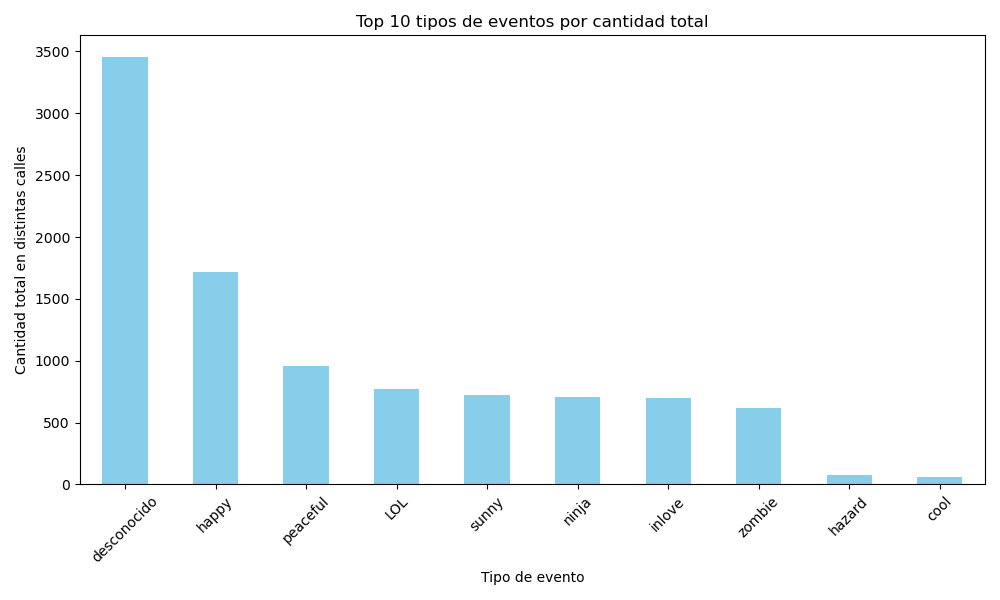
\includegraphics[width=0.85\textwidth]{distribucion_tipos_evento.png}
    \caption{Distribución de tipos de evento almacenados}
\end{figure}

\textbf{Análisis:} El gráfico presenta los tipos de eventos más comunes registrados durante el scraping. El eje X indica las categorías de eventos extraídas desde Waze (como \texttt{hazard}, \texttt{accident}, \texttt{jam}, etc.), mientras que el eje Y representa la frecuencia con la que aparecen. Esta distribución entrega una visión clara sobre cuáles son los incidentes más recurrentes en la Región Metropolitana, información valiosa para definir futuras estrategias de optimización del caché y priorización de datos.


\section{Extras y funcionalidades adicionales}

\subsection{CRUD Interno Simulado}

Durante el scraping, se implementaron operaciones equivalentes a un CRUD:

\begin{itemize}
    \item \textbf{Create:} inserción de eventos en tiempo real
    \item \textbf{Read:} consulta desde Redis o MySQL
    \item \textbf{Update:} actualización del TTL de la caché
    \item \textbf{Delete:} limpieza manual del caché o limpieza por expiración automática
\end{itemize}

\subsection{Dockerización completa del sistema}

Todos los servicios fueron dockerizados utilizando un archivo \texttt{docker-compose.yml}, el cual define dos contenedores:

\begin{itemize}
    \item \texttt{mysql\_eventos}: Base de datos MySQL
    \item \texttt{redis\_cache}: Servicio Redis
\end{itemize}

El entorno no incluye un contenedor de aplicación, ya que el código Python es ejecutado desde el notebook \texttt{Tarea1.ipynb} o el script \texttt{funciones.py} directamente en el host.

Para asegurar la instalación de todas las dependencias, se utilizó un archivo \texttt{requirements.txt} con los paquetes necesarios:

\begin{itemize}
    \item \texttt{mysql-connector-python}
    \item \texttt{redis}
    \item \texttt{pandas, numpy, matplotlib}
    \item \texttt{openpyxl}
\end{itemize}

\section{Análisis y Discusión}

\subsection{Generador de Tráfico}

Se utilizaron las distribuciones Poisson y Exponencial debido a que son modelos ampliamente usados para simular tiempos entre llegadas en sistemas de colas, redes de telecomunicaciones y tráfico. Estas distribuciones son realistas, ya que el tráfico de usuarios no es constante ni determinista, sino que sigue patrones probabilísticos.

Las simulaciones implementadas consisten en 100 consultas distribuidas sobre 10 eventos únicos, generando 10 repeticiones por evento. Este escenario representa un caso de alta repetición, lo cual es común en sistemas de información vial en tiempo real, como Waze, donde un mismo incidente puede ser consultado por miles de usuarios en un periodo corto de tiempo, especialmente en horas punta o ante situaciones críticas (como accidentes o cortes de ruta).

Este tipo de simulación busca validar la efectividad del sistema de caché ante patrones de acceso intensivos a un subconjunto reducido de datos, permitiendo evaluar la utilidad de Redis en contextos donde la mayoría de las consultas apuntan a los mismos registros.

Las métricas utilizadas para evaluar el rendimiento fueron:

\begin{itemize}
    \item \textbf{Número total de aciertos (hits)}: cuando el dato ya está en caché.
    \item \textbf{Número total de fallos (misses)}: cuando se tuvo que consultar a la base de datos.
    \item \textbf{Porcentaje de efectividad acumulada del caché}: mide el rendimiento conforme avanza la simulación.
\end{itemize}

\subsubsection*{Consideraciones para futuras pruebas}

Aunque las pruebas actuales permiten observar el impacto de Redis en un escenario de tráfico repetitivo, es recomendable ampliar el conjunto de pruebas incluyendo:

\begin{itemize}
    \item \textbf{Consultas aleatorias}: sobre eventos distribuidos uniformemente, para simular patrones de acceso menos concentrados.
    \item \textbf{Variación de la cantidad de eventos y repeticiones}: para observar el comportamiento del sistema ante consultas dispersas o muy masivas.
    \item \textbf{Medición del tiempo promedio de respuesta}: para complementar las métricas de efectividad con tiempos reales de acceso.
\end{itemize}

Estas pruebas permitirán robustecer la validación del sistema y ajustar mejor las políticas de caché ante escenarios dinámicos y reales.


\subsection{Almacenamiento}

Se utilizó \texttt{MySQL} como sistema de almacenamiento principal debido a su madurez, eficiencia y compatibilidad con múltiples herramientas, incluyendo contenedores Docker, Python (conectores), y Jupyter. Permite realizar consultas estructuradas mediante SQL y ofrece un rendimiento sólido para operaciones de lectura frecuente.

Se consideraron otras alternativas como \texttt{MongoDB}, pero fueron descartadas por su complejidad adicional al manejar esquemas flexibles y consultas no relacionales, lo cual no aportaba valor en este escenario donde los eventos tienen una estructura tabular fija. Además, \texttt{MySQL} facilita la exportación de resultados a hojas de cálculo, lo cual fue útil en las fases de análisis y visualización.

Una limitación conocida de \texttt{MySQL} es su escalabilidad vertical. Sin embargo, para el alcance de esta entrega y la cantidad de eventos manejados (aproximadamente 10.000), su rendimiento fue más que suficiente. En entregas futuras, se evaluará la posibilidad de migrar a soluciones escalables horizontalmente si se requiere análisis en tiempo real o con mayor volumen de datos.


\subsection{Métricas y Políticas de Caché}

El sistema de caché fue implementado utilizando \texttt{Redis} debido a su alta velocidad, simplicidad de integración con Python y soporte nativo para operaciones tipo \texttt{key-value}. Redis opera en memoria, lo que garantiza tiempos de respuesta mínimos, especialmente valioso en sistemas donde las consultas repetitivas deben ser atendidas rápidamente.

Para esta entrega, se utilizó una política de expiración basada en \textbf{TTL (Time To Live)} con una duración fija de 3600 segundos (1 hora). Esta decisión se tomó por su facilidad de configuración y porque Redis la implementa de manera nativa sin requerir lógica adicional. TTL permite purgar automáticamente los datos que ya no son recientes, evitando así el crecimiento descontrolado del caché.

No obstante, existen otras políticas de reemplazo más sofisticadas que podrían ofrecer mejores resultados en contextos con patrones de tráfico heterogéneos. Por ejemplo:

\begin{itemize}
    \item \textbf{LRU (Least Recently Used):} elimina los elementos menos utilizados recientemente. Es útil cuando se espera que ciertos eventos se consulten frecuentemente en intervalos cortos.
    \item \textbf{LFU (Least Frequently Used):} elimina los elementos menos consultados. Se adapta mejor a cargas donde algunas consultas dominan el tráfico.
\end{itemize}

Para comparar, se podría implementar una métrica adicional como la \textit{tasa de reemplazo} o medir el tiempo promedio de respuesta bajo distintas políticas. Dado el comportamiento repetitivo simulado en esta entrega, TTL resultó adecuado, pero en sistemas reales donde los patrones de acceso varían dinámicamente, LRU o LFU podrían ofrecer un mejor rendimiento.

Las métricas utilizadas para evaluar el caché fueron:

\begin{itemize}
    \item Porcentaje de aciertos (\texttt{hits})
    \item Porcentaje de fallos (\texttt{misses})
    \item Efectividad acumulada del caché a lo largo del tiempo
\end{itemize}

Con estas métricas, se evidenció una efectividad de entre 90\% y 91\%, validando el impacto positivo de Redis bajo los escenarios simulados.

\subsubsection*{Justificación del uso de TTL}

La política de \textbf{TTL (Time To Live)} fue utilizada para simplificar la gestión del caché. Cada evento almacenado en Redis permanece disponible durante un tiempo determinado (1 hora en este caso), tras el cual se elimina automáticamente sin necesidad de intervención manual.

Esta estrategia es adecuada en escenarios donde los datos pierden relevancia rápidamente —por ejemplo, eventos de tráfico que solo son relevantes durante un período corto—. Sin embargo, TTL no considera si un dato fue consultado muchas veces o si es particularmente popular. Simplemente elimina cualquier entrada al vencer su tiempo de vida.

\textbf{Reflexión:} TTL es una política simple, pero no adaptativa. Si el patrón de tráfico varía o ciertos eventos se vuelven altamente consultados en momentos específicos, TTL puede terminar eliminando entradas aún relevantes. En cambio, políticas como \textbf{LRU} o \textbf{LFU} permiten conservar los eventos más populares y ajustarse mejor a comportamientos dinámicos.

\subsubsection*{Comparación de políticas de reemplazo}

\begin{table}[H]
    \centering
    \begin{tabular}{|c|p{4.5cm}|p{4.5cm}|}
        \hline
        \textbf{Política} & \textbf{Ventaja} & \textbf{Desventaja} \\
        \hline
        TTL & Simple, fácil de implementar y mantener & No considera popularidad ni frecuencia de uso \\
        \hline
        LRU & Se adapta al uso real, manteniendo datos recientemente consultados & Requiere seguimiento del orden de acceso, más compleja \\
        \hline
        LFU & Conserva los elementos más frecuentemente usados & Puede penalizar nuevos datos si hay poco historial \\
        \hline
    \end{tabular}
    \caption{Comparación de políticas de reemplazo de caché}
\end{table}

Para esta entrega se optó por TTL debido a su simplicidad y porque Redis lo soporta nativamente sin configuración avanzada. En futuras versiones del sistema, se evaluará implementar y comparar estas políticas usando herramientas como \texttt{Redis eviction policies} o librerías personalizadas en Python, con el fin de adaptar mejor la retención de datos a distintos perfiles de tráfico urbano.



\section{Conclusiones}

El desarrollo de esta entrega permitió consolidar una arquitectura funcional distribuida que resuelve de manera efectiva el desafío de extracción y análisis de eventos de tráfico a gran escala. A través de la implementación modular de scraping, almacenamiento, generación de tráfico sintético y sistema de caché, se logró cumplir con todos los requisitos establecidos en la pauta del proyecto.

Uno de los aprendizajes más relevantes fue la validación empírica del uso de Redis como sistema de cacheo. Los resultados obtenidos mostraron una mejora significativa en la eficiencia de las consultas repetidas, con un \textbf{90-91\% de efectividad en cache} en escenarios simulados de 100 consultas sobre 10 eventos únicos. Esta alta tasa de hits demostró el impacto directo que puede tener una buena estrategia de caching sobre el rendimiento general del sistema.

El uso de distribuciones estadísticas (Poisson y Exponencial) para el modelado de tráfico de consultas fue crucial para simular condiciones realistas de acceso concurrente. Estas distribuciones representan correctamente contextos donde la llegada de eventos puede ser variable, como sucede en sistemas urbanos dinámicos. Además, su integración permitió contrastar el comportamiento del caché en distintos patrones de carga.

Desde el punto de vista de infraestructura, la dockerización de los servicios MySQL y Redis permitió garantizar portabilidad y replicabilidad del entorno, facilitando su uso en distintos equipos y futuras entregas. El uso de Jupyter como entorno de experimentación también potenció la visibilidad y trazabilidad del proceso, en paralelo al script Python que automatiza tareas.

Finalmente, el proyecto cumplió con la meta de construir una base robusta para las futuras etapas del sistema distribuido. La información recolectada, la arquitectura implementada y los mecanismos de prueba sentaron las bases para incorporar nuevas funcionalidades como procesamiento de datos, visualización avanzada y escalabilidad horizontal.

\newpage
\section{Referencias}
\begin{itemize}
    \item \href{https://docs.docker.com/compose/}{Docker Compose Documentation}
    \item \href{https://redis.io/docs/}{Redis Documentation}
    \item \href{https://dev.mysql.com/doc/}{MySQL Reference Manual}
    \item \href{https://numpy.org/}{NumPy}
    \item \href{https://matplotlib.org/}{Matplotlib}
\end{itemize}

\newpage
\section{Entrega del Proyecto}

A continuación, se indican los enlaces correspondientes a la entrega oficial del proyecto:

\begin{itemize}
    \item \textbf{Project ID:} \texttt{69384236}
    
    \item \textbf{Repositorio general del curso (GitLab):} \\
    \href{https://gitlab.com/proyectos_u/sistemas_distribuidos}{\texttt{https://gitlab.com/proyectos\_u/sistemas\_distribuidos}}

    \item \textbf{Repositorio del grupo con commit específico:} \\
    \href{https://gitlab.com/proyectos_u/sistemas_distribuidos/-/tree/629a4e1f1053e4978d748cdd4e3b2c96d7af5ff3/}{\texttt{629a4e1f1053e4978d748cdd4e3b2c96d7af5ff3}}

  
\end{itemize}

\end{document}
